\section{Datasets as a Holistic Motivating Context}

I propose using datasets as a motivating introductory computing context.
As established in the previous subsection, this is not a novel approach -- upper forms have always historically used datasets and recently lower forms have started too.
However, there is very little evaluation of the success of this approach, and numerous roadblocks exist in using this context.
For my dissertation, I will investigate what technology and pedagogy can be used to take full advantage of this context according to a number of constraints.
Before describing what I have done and will do, however, this section will describe this context in more detail.

\begin{wrapfigure}{r}{0.5\textwidth}
    \begin{center}
		    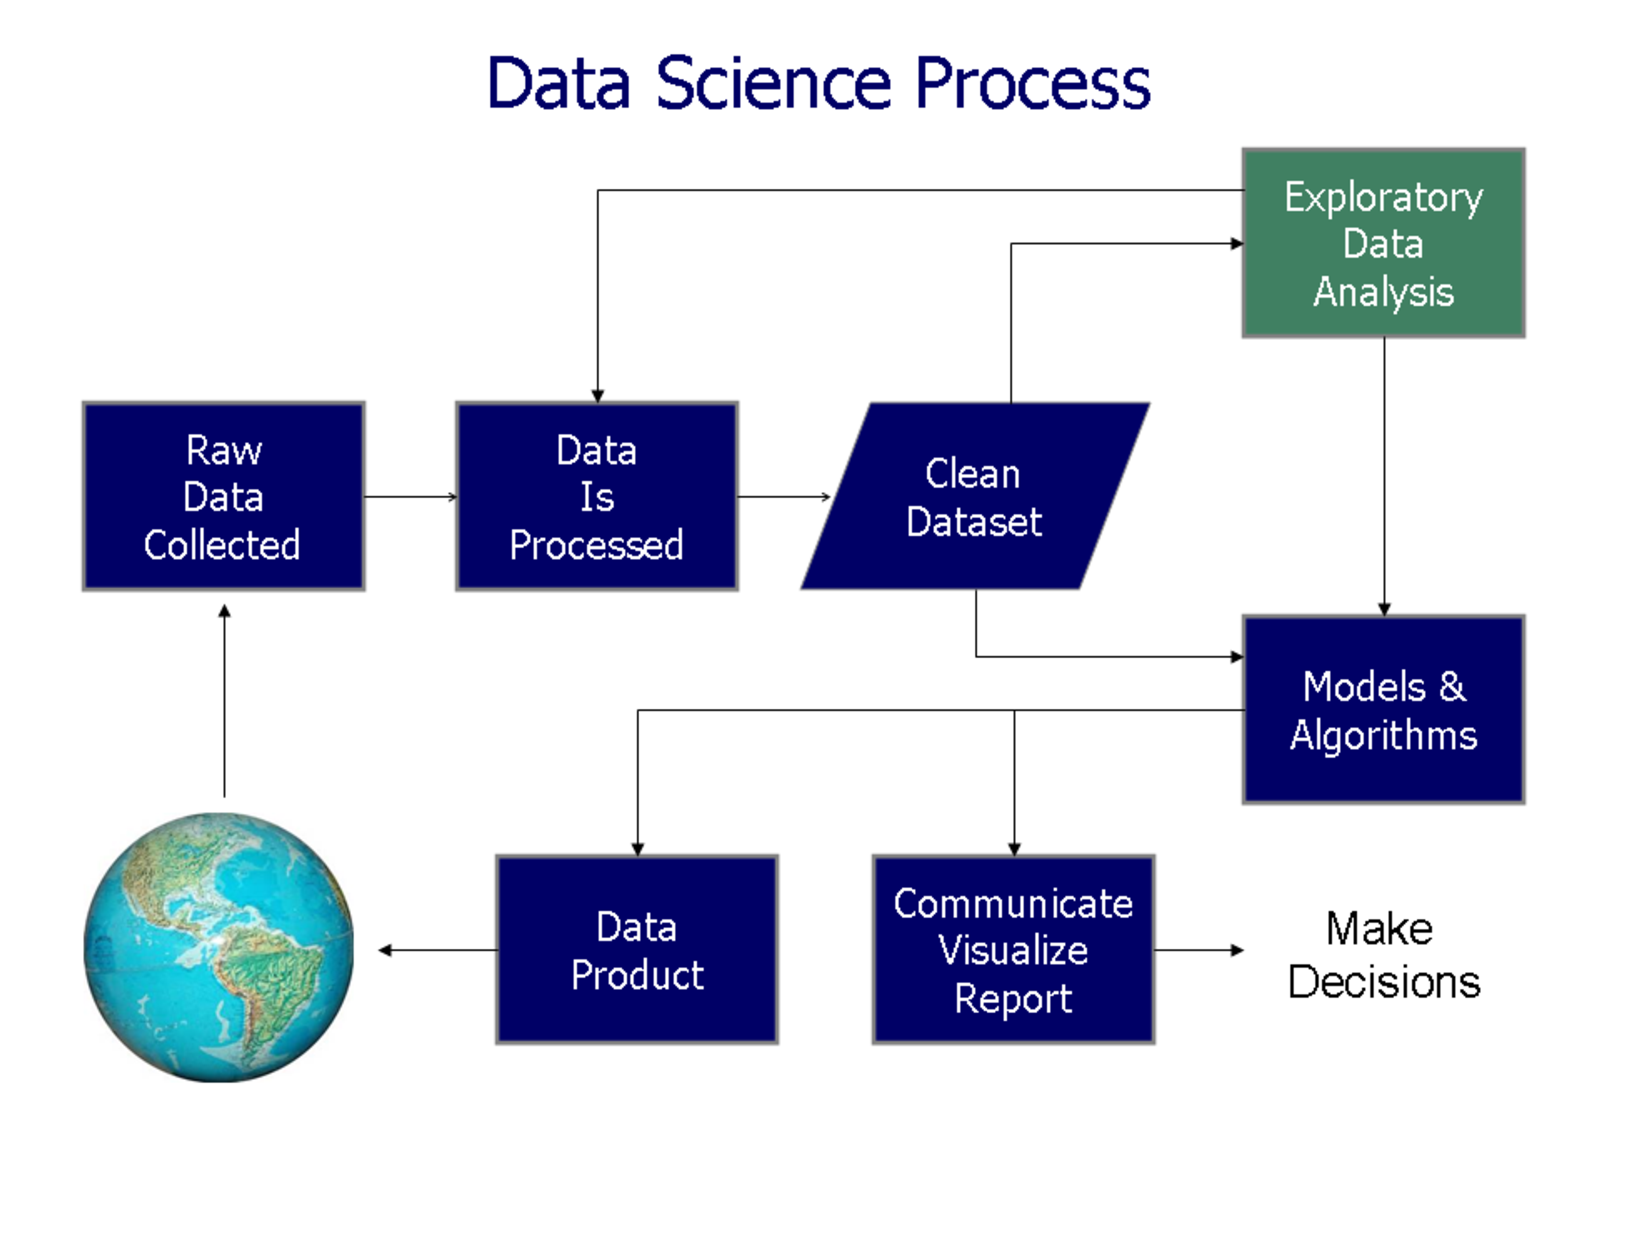
\psfig{file=images/data-science.eps, width=\linewidth}
    \end{center}
    \vspace{-\bigskipamount}
    \caption{A generalized model of Data Science\protect\cite{data-science-diagram}}
    \label{fig-data-science}
\end{wrapfigure}

Data science is the process of answering questions by building, exploring, and processing datasets.
There are many theoretical models that define the term more strictly, but in general it is described as an iterative model of collecting, sanitizing, processing, rendering, and interpreting.
Figure \ref{fig-data-science} gives a visual overview of this process.
My research will not attempt to narrowly define data science; instead, the goal is simply to use elements of the data science process.

It is crucial to understand that the goal is not to teach students how to become data scientists, anymore than it is the goal of Media Computation to teach students how to be professional computational artists.
As a context, using datasets is simply a means to an end -- it may involve any components of the generalized data science process at any level.
Some professors may identify data science as a learning objective in and of itself. That is fine, but they are attempting to teach something that is, at some level, distinct from computing itself.

My core thesis is that data science, used properly, is an excellent context for motivating students across all possible factors of motivation: providing opportunities for agency, a sense of usefulness and authenticity, controllable complexity, the potential to be interesting situationally and towards individualized interest, and a promotion of caring and ethics.
Data Science accomplishes this by being a ``meta-context'' -- it is a general framework for working with an infinitely wide array of different data contexts.
However, there are many challenges in doing so.

\subsection{Big Data}

One large categorization of data is Big Data. Big Data is much in the news these days, from reports of massive data
dredging by the NSA to tens of millions of credit cards stolen by
hackers from commercial databases.
Big Data has become crucial to scientific advances from understanding the
genome to predicting climate change.
Even more so than regular data science, there are many obstacles to effectively educating students on Big
Data.
Its representation, manipulation, and expression is, by definition, challenging, and modern curriculum and programming tools are typically inadequate.

\begin{wrapfigure}{r}{0.5\textwidth}
    \begin{center}
		    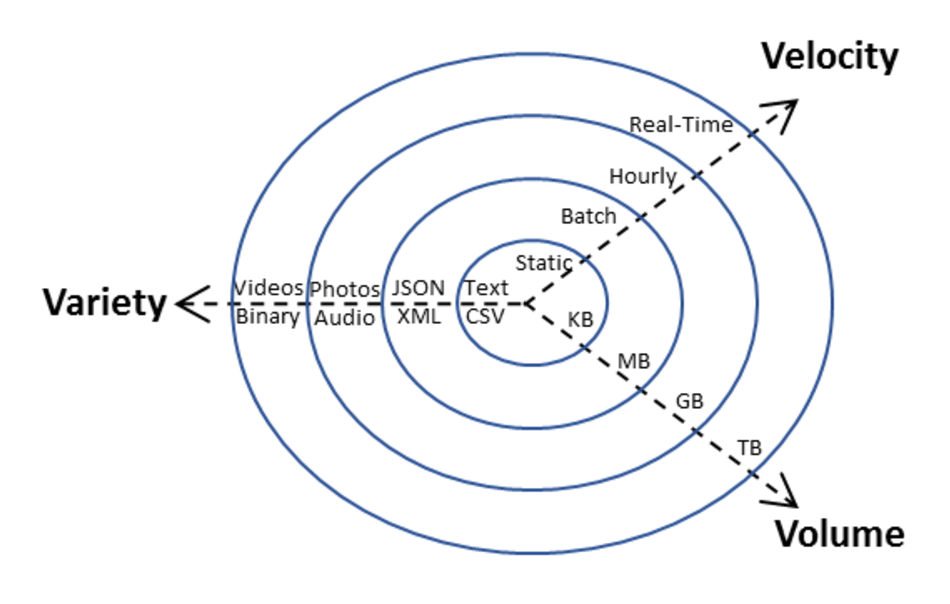
\psfig{file=images/3v-model.eps, width=\linewidth}
    \end{center}
    \vspace{-\bigskipamount}
    \caption{The 3V Model of Big Data}
    \label{fig-3v}
\end{wrapfigure}

Big data has been loosely described as quantities of information that cannot be handled with traditional methods ~\cite{McKinsey}.
But ``traditional methods'' is a vague phrase that has different meanings to different learners. To a Humanities major in their first CS-0 course, the traditional method to sum a list is to use Excel. In this scenario, ``big data'' means anything that won't comfortably fit into Excel's working memory.
However, to a third-year Computer Science major, the traditional method would be to write an iterative or recursive sequential loop; being given big data forces them to explore parallel models of execution.
Clearly, ``bigness'' is a function of the learner's experience, but that is still not a solid definition.
A more precise definition is the ``3V Model'' \cite{douglas2012importance}, which posits that there are three dimensions that distinguish big data from ordinary, run-of-the-mill data:

\begin{description}
	\item[Volume:] The total quantity of the information, usually measured in bytes or number of records. However, this also extends laterally: the number of fields in the structure of the data also impacts the complexity and size. The threshold at which data becomes big is a function of the hardware and software being used. For instance, embedded systems may consider gigabyte-sized files to be big, while modern servers might not struggle until the petabyte level.
	\item[Velocity:] The rate at which new information is added to the system. High velocity big data implies a distributed architecture, since new data must be arriving from somewhere. The dynamicity of data can vary widely across these architectures, with data updating every year, every day, or even multiple times a second.
	\item[Variety:] The format or formats of the data. Ideally, data are always distributed in a way that is readily accessible. For instance, simple text-based formats such as CSV and JSON are widely supported, relatively lightweight, and human-readable. More sophisticated data formats for image and audio are also typically well-supported, although still more complicated. However, projects using specialized, compressed binary formats or, more dangerously, multiple formats (e.g., image archives organized with XML files), are more complex.
\end{description}

Silva~\cite{Silva:2014} taught an introductory course truly focused on techniques for tackling Big Data: NoSQL, MapReduce, NewSQL.
Unfortunately, they did not conduct any kind of evaluation of their work across any of the expected dimensions. 
Learning to work with Big Data can add extra authenticity to the context, but it also raises a large number of new challenges.
Once again, it is not the goal of my research to teach students how to work with truly Big datasets. Instead, it is simply a means to motivate students.
In the following sections, I describe some specific challenges of working with Big Data, and the possible approaches to solving them.

\subsubsection{High Velocity Data}

It is not trivial to enable introductory students to work with high velocity data, which is necessarily distributed. Without any scaffolding, it is necessary to delay the use of such data until much later in the course. In a prior paper \cite{realtimeweb-splashe}, we outline the biggest barriers to high velocity data as a context:
\begin{description}
  \item[Access] The process of programmatically downloading and parsing a web-based resource is a non-trivial procedure requiring an understanding of both basic concepts (e.g., function calls, data transformation) and specialized web technology (e.g., the difference between GET and POST calls, building query parameters).
	\item[Non-Idempotency] Because high velocity data is constantly changing, repeated calls to the same URL endpoint can return wildly different results, even over the course of a few minutes. This makes finding errors and testing considerably harder.
	\item[Consistency] Web-based APIs are controlled and developed by independent entities, which means that changes can occur at any time with little to no notification or time for reaction. This means that students' code can become out of date even during the middle of testing their final project.
	\item[Connectivity] Although internet speeds for students on a university campus are typically stable, this does not extend to off-campus students or students that are traveling. If the internet connection is down, then students might be completely unable to make progress.
	\item[Efficiency] Even when the internet connection is stable, it might not always be fast. Requiring a round-trip to a server can greatly drag on the testing and development process, frustrating the student and decreasing the time spent learning.
\end{description}

\subsubsection{High Volume Data}

\begin{description}
	\item[Data Transmission:] Internet connections can be difficult and inconsistent, especially for off-campus
and non-traditional students. Although most modern universities boast impressive wired connection
speeds, these speeds rarely extend off-campus. And even when internet connections are top-notch,
they can still be inadequate to serving the needs of transmitting big data collections to an entire
classroom of students. Some affordances must be made to make the data readily available to students without taxing their hard drives unnecessarily.
	\item[Historically-oriented data:] Additionally, high volume data offers different contexts and problems than high velocity data.
For instance, high velocity data typically lends itself to small quantities of data that are relevant to the current state of the real world -- for instance, students can walk outside and feel the current weather, which should correlate to real-time weather reports made available by a weather library.
High volume data, on the other hand, lends itself to large quantities of mostly static data -- for instance, crime reports for a long period of time.
Although high velocity data gives authentic answers in the here and now, high volume data gives authentic answers for the future, through trends.
Some fields have both kinds of data available -- meteorologists generate forecasts (high velocity, low volume) by studying historical climate data (high volume, low velocity).
But some fields are not amenable to both -- digital historians typically have large stores of historical information (high volume), but it does not change quickly (low velocity).
Careful consideration must be made when choosing problems and designing contexts so that the data leads to optimally authentic learning experiences.
\end{description}


\subsubsection{High Variety Data}

\begin{description}
\item[Inconsistency of Storage:] High variety data is composed of many different kinds of file formats -- some of which are more complicated than others.
\item[Inconsistency of Tools:] Different languages usually offer many different tools to interact with the exotic formats of the data. However, these tools vary greatly in availability, usability, and compatibility across platforms. For instance, binary image data is supported as a first-class programming object in the Racket programming environment, but can only be loaded using libraries such as Pygame in Python, which the user may or may not have installed.
\end{description}
